\documentclass[12pt]{beamer}
\usetheme{Madrid}

\usepackage{circuitikz}
\usepackage{amsmath, amssymb}
\usepackage{tikz}
\usetikzlibrary{arrows.meta, shapes.geometric}
\usepackage{xcolor}
\usepackage{bm}
\usepackage{listings}
\usepackage{courier}

\lstset{
  basicstyle=\ttfamily\scriptsize,
  breaklines=true,
  frame=single,
  columns=fullflexible
}

\setbeamerfont{frametitle}{series=\bfseries, size=\large}
\setbeamerfont{title}{series=\bfseries, size=\Large}
\setbeamerfont{subtitle}{series=\bfseries}

\definecolor{madblue}{RGB}{0,62,126}
\definecolor{okgreen}{RGB}{0,130,60}

%% TOC-style circled option
\newcommand{\myopt}[2]{%
  \vspace{5pt}\noindent
  \begin{tikzpicture}[baseline=(ch.base)]
    \node[circle, fill=madblue, text=white,
          font=\bfseries\small, minimum size=17pt, inner sep=0pt] (ch) {#1};
  \end{tikzpicture}
  \hspace{5pt}\textbf{#2}\par
}

\newcommand{\rarrow}{\textcolor{madblue}{$\boldsymbol{\Rightarrow}$}\;}

\title{\bfseries Transient Analysis of an RC Circuit}
\subtitle{\textbf{Problem 1.1.16 \;|\; EC 2007}}
\author{}
\institute{\textbf{EE25BTECH11016- CH. Taraka Abhinav}}
\date{}

\begin{document}

%% ── TITLE ────────────────────────────────────────────────────────
\begin{frame}
  \titlepage
\end{frame}

%% ── QUESTION ─────────────────────────────────────────────────────
\begin{frame}{\textbf{Problem 1.1.16 \;--\; EC 2007}}

\textbf{In the circuit shown,} $\bm{V_C = 0}$ \textbf{V at}
$\bm{t=0}$ \textbf{sec. For} $\bm{t>0}$\textbf{, the capacitor current}
$\bm{i_c(t)}$ \textbf{(}$\bm{t}$ \textbf{in seconds) is:}

\vspace{1em}

\begin{columns}[c]

    %% LEFT → OPTIONS
    \begin{column}{0.45\textwidth}
        {\textbf{\textcolor{madblue}{Options:}}}\\[0.4em]

        \myopt{a}{$0.50\,e^{-25t}\ \mathrm{mA}$}
        \myopt{b}{$0.25\,e^{-25t}\ \mathrm{mA}$}
        \myopt{c}{$0.50\,e^{-12.5t}\ \mathrm{mA}$}
        \myopt{d}{$0.25\,e^{-6.25t}\ \mathrm{mA}$}
    \end{column}

    %% RIGHT → CIRCUIT
    \begin{column}{0.55\textwidth}
        \centering
        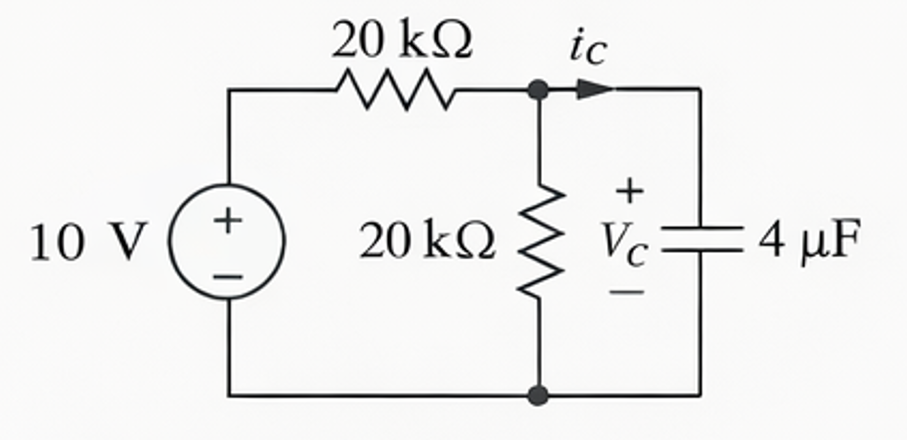
\includegraphics[width=\linewidth]{figs/C.png}
    \end{column}

\end{columns}

\end{frame}

%% ── SOLUTION 1: Initial Condition ────────────────────────────────
\begin{frame}{\textbf{Initial Condition}}
  \begin{center}
    \vfill
    \textbf{Given:}\quad $V_C(t=0^-) = 0\,\mathrm{V}$

    \vspace{1.2em}
    A capacitor \textbf{cannot change its voltage instantaneously}\\[0.4em]
    because an instantaneous change requires \textbf{infinite current},\\[0.4em]
    which is physically impossible.

    \vspace{1.5em}
    Therefore:
    \[
      V_C(t=0^+) \;=\; V_C(t=0^-) \;=\; \mathbf{0\,V}
    \]

    \vspace{0.6em}
    At $t = 0^+$, since $V_C = 0$, the capacitor behaves as a \textbf{short circuit}.
    \vfill
  \end{center}
\end{frame}

%% ── SOLUTION 2: Steady-State Voltage ─────────────────────────────
\begin{frame}{\textbf{Steady-State Voltage $V_\infty$}}
  \begin{center}
    \vfill
    As $t \to \infty$, the capacitor is \textbf{fully charged}\\[0.4em]
    \rarrow no current flows into it \rarrow capacitor is an \textbf{open circuit}

    \vspace{1.2em}
    The two resistors then form a simple \textbf{Voltage Divider}:

    \vspace{0.8em}
    \[
      V_\infty \;=\; V_s \times \frac{R_2}{R_1 + R_2}
              \;=\; 10 \times \frac{20\,\mathrm{k}}{20\,\mathrm{k} + 20\,\mathrm{k}}
              \;=\; 10 \times \frac{1}{2}
    \]

    \vspace{1em}
    \Large\textbf{\textcolor{madblue}{$V_\infty \;=\; 5\,\mathrm{V}$}}
    \vfill
  \end{center}
\end{frame}

%% ── SOLUTION 3: Thevenin Resistance ──────────────────────────────
\begin{frame}{\textbf{Thévenin Resistance $R_{th}$}}
  \begin{center}
    \vfill
    \textbf{Deactivate} the independent voltage source\\[0.3em]
    (replace with a \textbf{short circuit})

    \vspace{1em}
    Looking from the capacitor terminals, both $20\,\mathrm{k}\Omega$ resistors\\[0.3em]
    are now connected \textbf{in parallel}:

    \vspace{0.8em}
    \[
      R_{th} \;=\; 20\,\mathrm{k} \;\|\; 20\,\mathrm{k}
             \;=\; \frac{20 \times 20}{20 + 20}\,\mathrm{k}
             \;=\; \frac{400}{40}\,\mathrm{k}
    \]

    \vspace{1em}
    \Large\textbf{\textcolor{madblue}{$R_{th} \;=\; 10\,\mathrm{k}\Omega$}}
    \vfill
  \end{center}
\end{frame}

%% ── SOLUTION 4: Time Constant ────────────────────────────────────
\begin{frame}{\textbf{Time Constant $\tau$}}
  \begin{center}
    \vfill
    The time constant for an RC circuit is:
    \[
      \tau \;=\; R_{th} \cdot C
    \]

    \vspace{0.8em}
    Substituting $R_{th} = 10\,\mathrm{k}\Omega$ and $C = 4\,\mu\mathrm{F}$:
    \[
      \tau \;=\; 10 \times 10^{3} \;\times\; 4 \times 10^{-6}
           \;=\; 40 \times 10^{-3}\,\mathrm{s}
    \]

    \vspace{0.8em}
    \large\textbf{\textcolor{madblue}{$\tau \;=\; 40\,\mathrm{ms}$}}

    \vspace{1em}
    Therefore the decay exponent:
    \[
      \frac{1}{\tau} \;=\; \frac{1}{0.04} \;=\; \mathbf{25\,s^{-1}}
    \]
    \vfill
  \end{center}
\end{frame}

%% ── SOLUTION 5: Capacitor Voltage ────────────────────────────────
\begin{frame}{\textbf{Capacitor Voltage $V_C(t)$}}
  \begin{center}
    \vfill
    The standard RC complete response formula:
    \[
      V_C(t) \;=\; V_\infty \;+\; \bigl[V_C(t=0^+) - V_\infty\bigr]\,e^{-t/\tau}
    \]

    \vspace{0.8em}
    Substituting $V_\infty = 5\,\mathrm{V}$,\quad $V_C(t=0^+) = 0\,\mathrm{V}$,\quad $1/\tau = 25$:
    \[
      V_C(t) \;=\; 5 \;+\; [0 - 5]\,e^{-25t}
    \]

    \vspace{1em}
    \Large\textbf{\textcolor{madblue}{$V_C(t) \;=\; 5\bigl(1 - e^{-25t}\bigr)\,\mathrm{V}$}}

    \vspace{1.2em}
    \normalsize
    \textbf{Check:}\quad
    At $t=0$:\; $V_C = 5(1-1) = 0\,\mathrm{V}$ \;\textcolor{okgreen}{\checkmark}
    \qquad
    As $t\to\infty$:\; $V_C \to 5\,\mathrm{V}$ \;\textcolor{okgreen}{\checkmark}
    \vfill
  \end{center}
\end{frame}

%% ── SOLUTION 6: Capacitor Current ────────────────────────────────
\begin{frame}{\textbf{Capacitor Current $i_c(t)$}}
  \begin{center}
    \vfill
    Using the fundamental capacitor relation:
    \[
      i_c(t) \;=\; C\,\frac{dV_C}{dt}
    \]

    \vspace{0.6em}
    Differentiating $V_C(t) = 5(1 - e^{-25t})$:
    \[
      \frac{dV_C}{dt} \;=\; 5 \times 25\,e^{-25t} \;=\; 125\,e^{-25t}\,\mathrm{V/s}
    \]

    \vspace{0.6em}
    Multiplying by $C = 4 \times 10^{-6}\,\mathrm{F}$:
    \[
      i_c(t) \;=\; 4\times10^{-6} \;\times\; 125\,e^{-25t}
              \;=\; 500\times10^{-6}\,e^{-25t}\,\mathrm{A}
    \]

    \vspace{1em}
    \LARGE\textbf{\textcolor{madblue}{$i_c(t) \;=\; 0.50\,e^{-25t}\,\mathrm{mA}$}}
    \vfill
  \end{center}
\end{frame}

%% ── SOLUTION 7: KCL Verification ─────────────────────────────────
\begin{frame}{\textbf{Verification via KCL}}
  \begin{center}
    \vfill
    At the junction node, applying KCL:
    \[
      i_c \;=\; \underbrace{\frac{10 - V_C}{20\,\mathrm{k}}}_{i_1\text{ (series R)}}
               \;-\;
               \underbrace{\frac{V_C}{20\,\mathrm{k}}}_{i_2\text{ (shunt R)}}
             \;=\; \frac{10 - 2V_C}{20\,\mathrm{k}}
    \]

    \vspace{0.8em}
    Substituting $V_C = 5(1 - e^{-25t})$, so $\;2V_C = 10(1 - e^{-25t})$:
    \[
      i_c(t) \;=\; \frac{10 - 10(1 - e^{-25t})}{20\,\mathrm{k}}
              \;=\; \frac{10\,e^{-25t}}{20\,\mathrm{k}}
    \]

    \vspace{1em}
    \Large\textbf{\textcolor{madblue}{$i_c(t) \;=\; 0.50\,e^{-25t}\,\mathrm{mA}$}}
    \vfill
  \end{center}
\end{frame}
%% ── VOLTAGE: PYTHON ─────────────────────────────────────────────
\begin{frame}[fragile,allowframebreaks]{Capacitor Voltage -- Python}
\begin{lstlisting}
import numpy as np
import matplotlib.pyplot as plt

t = np.linspace(0, 0.2, 1000)
V = 5
tau = 0.04

Vc = V*(1 - np.exp(-t/tau))

plt.plot(t*1000, Vc)
plt.axhline(5, linestyle='--')
plt.show()
\end{lstlisting}
\end{frame}

%% ── VOLTAGE: C CODE ─────────────────────────────────────────────
\begin{frame}[fragile,allowframebreaks]{Capacitor Voltage -- C Code}
\begin{lstlisting}
#include <stdio.h>
#include <math.h>

int main(){
    double t, V=5, tau=0.04;

    for(int i=0;i<=200;i++){
        t = i/1000.0;
        double Vc = V*(1-exp(-t/tau));

        printf("%lf %lf\n", t*1000, Vc);
    }
    return 0;
}
\end{lstlisting}
\end{frame}

%% ── VOLTAGE: PLOT ───────────────────────────────────────────────
\begin{frame}{Capacitor Voltage Plot}
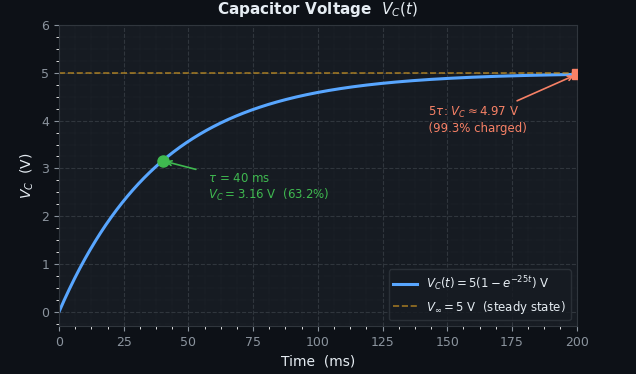
\includegraphics[width=\linewidth]{figs/Vc.png}
\end{frame}

%% ── CURRENT: PYTHON ─────────────────────────────────────────────
\begin{frame}[fragile,allowframebreaks]{Capacitor Current -- Python}
\begin{lstlisting}
import numpy as np
import matplotlib.pyplot as plt

t = np.linspace(0, 0.2, 1000)
V = 5
R = 10000
tau = 0.04

ic = (V/R)*np.exp(-t/tau)*1000

plt.plot(t*1000, ic)
plt.axhline(0, linestyle='--')
plt.show()
\end{lstlisting}
\end{frame}

%% ── CURRENT: C CODE ─────────────────────────────────────────────
\begin{frame}[fragile,allowframebreaks]{Capacitor Current -- C Code}
\begin{lstlisting}
#include <stdio.h>
#include <math.h>

int main(){
    double t, V=5, R=10000, tau=0.04;

    for(int i=0;i<=200;i++){
        t = i/1000.0;
        double ic = (V/R)*exp(-t/tau)*1000;

        printf("%lf %lf\n", t*1000, ic);
    }
    return 0;
}
\end{lstlisting}
\end{frame}

%% ── CURRENT: PLOT ───────────────────────────────────────────────
\begin{frame}{Capacitor Current Plot}
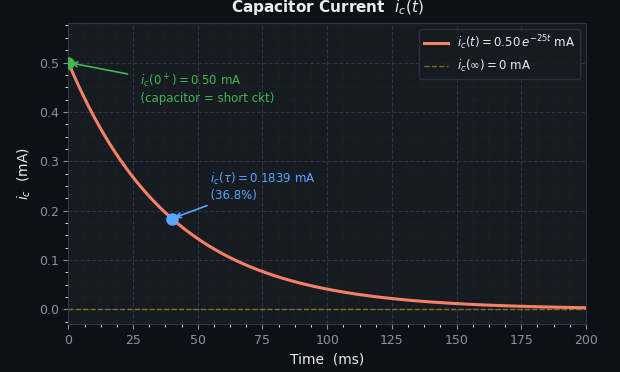
\includegraphics[width=\linewidth]{figs/Ic.png}
\end{frame}

%% ── OVERLAY: PYTHON ─────────────────────────────────────────────
\begin{frame}[fragile,allowframebreaks]{Overlay Plot -- Python Code}
\begin{lstlisting}
import numpy as np
import matplotlib.pyplot as plt

t = np.linspace(0, 0.2, 1000)
V = 5
tau = 0.04

Vc = V * (1 - np.exp(-t/tau))
ic = (V/10000) * np.exp(-t/tau) * 1000

fig, ax1 = plt.subplots()

ax1.plot(t*1000, Vc)
ax1.set_xlabel("Time (ms)")
ax1.set_ylabel("Vc (V)")

ax2 = ax1.twinx()
ax2.plot(t*1000, ic, linestyle='--')
ax2.set_ylabel("ic (mA)")

plt.show()
\end{lstlisting}
\end{frame}

%% ── OVERLAY: C CODE ─────────────────────────────────────────────
\begin{frame}[fragile,allowframebreaks]{Overlay Plot -- C Code}
\begin{lstlisting}
#include <stdio.h>
#include <math.h>

int main() {
    double t, V=5, tau=0.04;

    for(int i=0;i<=200;i++){
        t = i/1000.0;
        double Vc = V*(1-exp(-t/tau));
        double ic = (V/10000.0)*exp(-t/tau)*1000;

        printf("%lf %lf %lf\n", t*1000, Vc, ic);
    }
    return 0;
}
\end{lstlisting}
\end{frame}

%% ── OVERLAY: PLOT ───────────────────────────────────────────────
\begin{frame}{Overlay Plot}
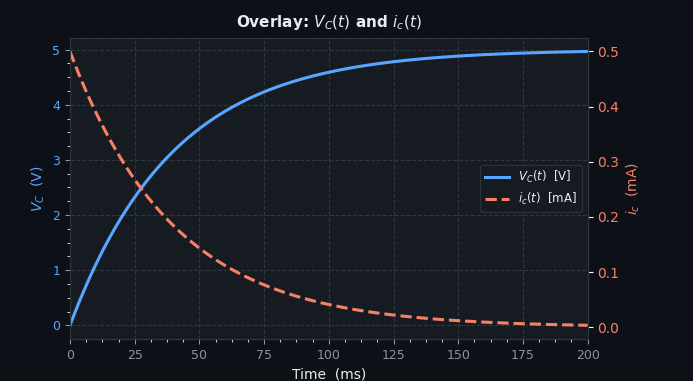
\includegraphics[width=\linewidth]{figs/O.png}
\end{frame}

\end{document}